% 本模板根据中国科学院大学本科生公共必修课程《基础物理实验》Word模板格式编写
% 本模板由Shing-Ho Lin和Jun-Xiong Ji于2022年9月共同完成, 旨在方便LaTeX原教旨主义者和被Word迫害者写实验报告, 避免Word文档因插入过多图与公式造成卡顿. 
% 如有任何问题, 请联系: linchenghao21@mails.ucas.ac.cn
% This is the LaTeX template for experiment report of Experimental Physics courses, based on its provided Word template. 
% This template is completed by the joint collabration of Shing-Ho Lin and Junxiong Ji in September 2022. 
% Adding numerous pictures and equations leads to unsatisfying experience in Word. Therefore LaTeX is better. 
% Feel free to contact us via: linchenghao21@mails.ucas.ac.cn

\documentclass[11pt]{article}

\usepackage[a4paper]{geometry}
\geometry{left=2.0cm,right=2.0cm,top=2.2cm,bottom=2.2cm}

\usepackage{ctex} % 支持中文的LaTeX宏包
\usepackage{amsmath,amsfonts,graphicx,subfigure,amssymb,bm,amsthm,mathrsfs,mathtools,breqn} % 数学公式和符号的宏包集合
\usepackage{algorithm,algorithmicx} % 算法和伪代码的宏包
\usepackage[noend]{algpseudocode} % 算法和伪代码的宏包
\usepackage{fancyhdr} % 自定义页眉页脚的宏包
\usepackage[framemethod=TikZ]{mdframed} % 创建带边框的框架的宏包
\usepackage{fontspec} % 字体设置的宏包
\usepackage{adjustbox} % 调整盒子大小的宏包
\usepackage{fontsize} % 设置字体大小的宏包
\usepackage{tikz,xcolor} % 绘制图形和使用颜色的宏包
\usepackage{multicol} % 多栏排版的宏包
\usepackage{multirow} % 表格中合并单元格的宏包
\usepackage{pdfpages} % 插入PDF文件的宏包
\RequirePackage{listings} % 在文档中插入源代码的宏包
\RequirePackage{xcolor} % 定义和使用颜色的宏包
\usepackage{wrapfig} % 文字绕排图片的宏包
\usepackage{bigstrut,multirow,rotating} % 支持在表格中使用特殊命令的宏包
\usepackage{booktabs} % 创建美观的表格的宏包
\usepackage{circuitikz} % 绘制电路图的宏包
\usepackage[inline]{enumitem}
\usepackage{tabularx}

\usepackage{indentfirst}
\setlength{\parindent}{2em}
\setlength{\abovecaptionskip}{2pt}
\setlength{\belowcaptionskip}{2pt}
\setlength{\intextsep}{8pt}
\setlength{\floatsep}{8pt}

\definecolor{dkgreen}{rgb}{0,0.6,0}
\definecolor{gray}{rgb}{0.5,0.5,0.5}
\definecolor{mauve}{rgb}{0.58,0,0.82}
\lstset{
  frame=tb,
  aboveskip=3mm,
  belowskip=3mm,
  showstringspaces=false,
  columns=flexible,
  framerule=1pt,
  rulecolor=\color{gray!35},
  backgroundcolor=\color{gray!5},
  basicstyle={\small\ttfamily},
  numbers=none,
  numberstyle=\tiny\color{gray},
  keywordstyle=\color{blue},
  commentstyle=\color{dkgreen},
  stringstyle=\color{mauve},
  breaklines=true,
  breakatwhitespace=true,
  tabsize=3,
}

% 轻松引用, 可以用\cref{}指令直接引用, 自动加前缀. 
% 例: 图片label为fig:1
% \cref{fig:1} => Figure.1
% \ref{fig:1}  => 1
\usepackage[capitalize]{cleveref}
% \crefname{section}{Sec.}{Secs.}
\Crefname{section}{Section}{Sections}
\Crefname{table}{Table}{Tables}
\crefname{table}{Table.}{Tabs.}

\setmainfont{Palatino Linotype.ttf}
\setCJKmainfont{SimHei.ttf}
% \setCJKsansfont{Songti.ttf}
% \setCJKmonofont{SimSun.ttf}
\punctstyle{kaiming}
% 偏好的几个字体, 可以根据需要自行加入字体ttf文件并调用

\renewcommand{\emph}[1]{\begin{kaishu}#1\end{kaishu}}

%改这里可以修改实验报告表头的信息
\newcommand{\experiName}{示波器,信号发生器}
\newcommand{\supervisor}{丰家峰}
\newcommand{\name}{张欣培}
\newcommand{\studentNum}{2022K8009922001}
\newcommand{\class}{01}
\newcommand{\group}{07}
\newcommand{\seat}{}
\newcommand{\dateYear}{2023}
\newcommand{\dateMonth}{9}
\newcommand{\dateDay}{18}
\newcommand{\room}{教709}
\newcommand{\others}{$\square$}
%% 如果是调课、补课, 改为: $\square$\hspace{-1em}$\surd$
%% 否则, 请用: $\square$
%%%%%%%%%%%%%%%%%%%%%%%%%%%

\begin{document}

%若需在页眉部分加入内容, 可以在这里输入
% \pagestyle{fancy}
% \lhead{\kaishu 测试}
% \chead{}
% \rhead{}

\begin{center}
    \LARGE \bf 《\, 基\, 础\, 物\, 理\, 实\, 验\, 》\, 实\, 验\, 报\, 告
\end{center}

\begin{center}
    \noindent \emph{实验名称}\underline{\makebox[25em][c]{\experiName}}
    \emph{指导教师}\underline{\makebox[8em][c]{\supervisor}}\\
    \emph{姓名}\underline{\makebox[6em][c]{\name}} 
    % 如果名字比较长, 可以修改box的长度"6em"
    \emph{学号}\underline{\makebox[10em][c]{\studentNum}}
    \emph{分班分组及座号} \underline{\makebox[5em][c]{\class \ -\ \group \ -\ \seat }\emph{号}} (\emph{例}:\, 1\,-\,04\,-\,5\emph{号})\\
    \emph{实验日期} \underline{\makebox[3em][c]{\dateYear}}\emph{年}
    \underline{\makebox[2em][c]{\dateMonth}}\emph{月}
    \underline{\makebox[2em][c]{\dateDay}}\emph{日}
    \emph{实验地点}\underline{{\makebox[4em][c]\room}}
    \emph{调课/补课} \underline{\makebox[3em][c]{\others\ 是}}
    \emph{成绩评定} \underline{\hspace{5em}}
    {\noindent}
    \rule[8pt]{17cm}{0.2em}
\end{center}

\begin{center}
    \Large \bf 第一部分\qquad 实验内容
\end{center}

\section{实验目的}

\begin{enumerate}
    \item 熟悉信号发生器和示波器的使用方法
    \item 了解示波器和信号发生器的一系列参数
    \item 使用信号发生器产生一系列稳定波形(正弦波或方波),用示波器观察
\end{enumerate}

\section{实验器材}

    \hspace*{2em} 信号发射器,数字储存示波器,稳压电源,示波器探头,同轴线等线材,发光二极管等电路元器件。

\section{实验原理}
\begin{enumerate}
    \item 信号发生器生成各种波形的电波。
    \item 示波器能将电子周期性打在屏幕上从而形成图像。本次使用数字储存示波器,能够将波形储存为数字信号后显示,方便观察、记录、操作。
    \item 万用电表能够测量直流电压、交流电压、电流、电阻等物理量。
\end{enumerate}


\section{实验内容}


\begin{enumerate}
    \item 设备的一些按钮及其功能
    \begin{enumerate}
        \item 函数发生器 \newline \hspace*{2em} 生成各种波形的信号,可调整的参数有频率、幅度、偏置、相位等。需要注意点有:CH1/CH2的选择,output打开。具体的调整依照仪器不同,不多赘述。其中mod,sweep,burst按钮功能能够产生更多效果的波形。
        \item 示波器 \newline \hspace*{2em} 显示函数发生器或外界生成的信号。auto按钮能够自适应其频率、振幅等信息,自动调整图像使其在合适的位置显示。我们也可以通过旋钮调整振幅、偏置等参数,这些调整只改变显示效果,不改变输入数据本身。其中math按钮内含的数学运算与逻辑运算具有重要价值。其他操作依设备而异。双线或多线连接时,按对应输入口按钮后进行调节。
              \newline \hspace*{2em} X/Y模式下,输出两输入之间的关系,产生李萨如图像。正弦波输入下,两周期为整数倍时,图像稳定。通过acquire按键打开X/Y模式。 
              \newline \hspace*{2em} utility调整阻抗,50Ω高频,高阻低频。
    \end{enumerate}
    \item 实验过程
    \begin{enumerate}
        \item 连接线路,启动示波器与函数发生器,自行调节参数,观察波形。
        \item 连接两输入输出,观察两波形,使用数学运算(此处是+)。
        \item 使用X/Y模式,观察李萨如图像。
        \item 使用roll模式(实验中我未保留图片)。
        \item 尝试信号发生器与示波器的阻抗设置。在测试中暂时没发现区别,可能是因为输入数据频率不够高/不够低。
        
        %下面是图片
        %\begin{figure}[H]
        %    \centering
        %    \begin{minipage}[t]{0.33\linewidth}
        %        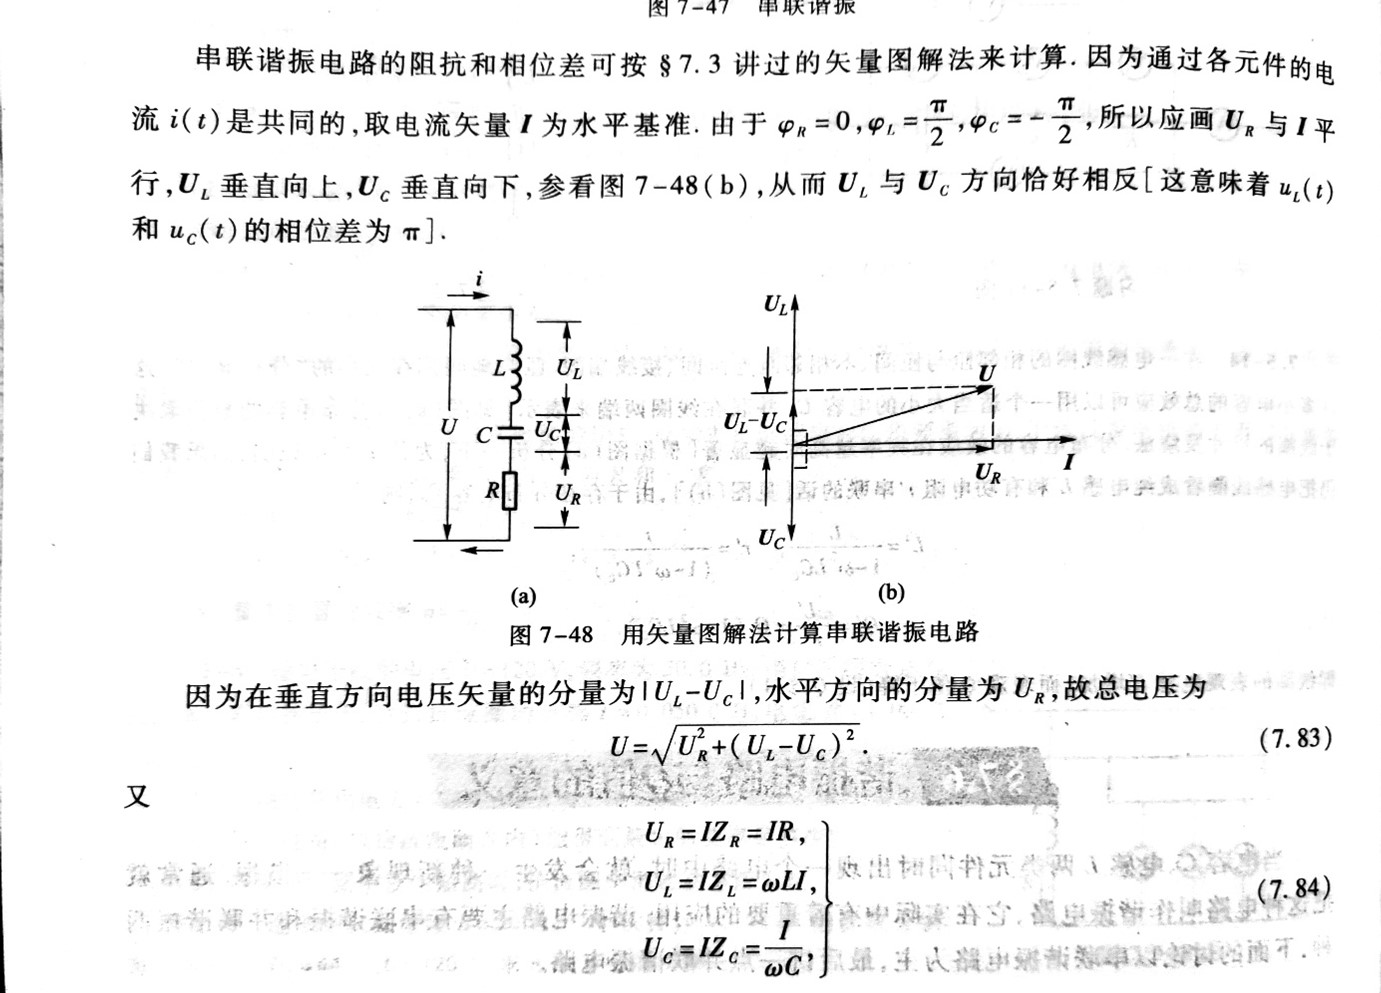
\includegraphics[width=5cm]{Fig/1.jpg}
        %        \caption{示波器显示-单波}
        %    \end{minipage}
        %    \begin{minipage}[t]{0.33\linewidth}
        %        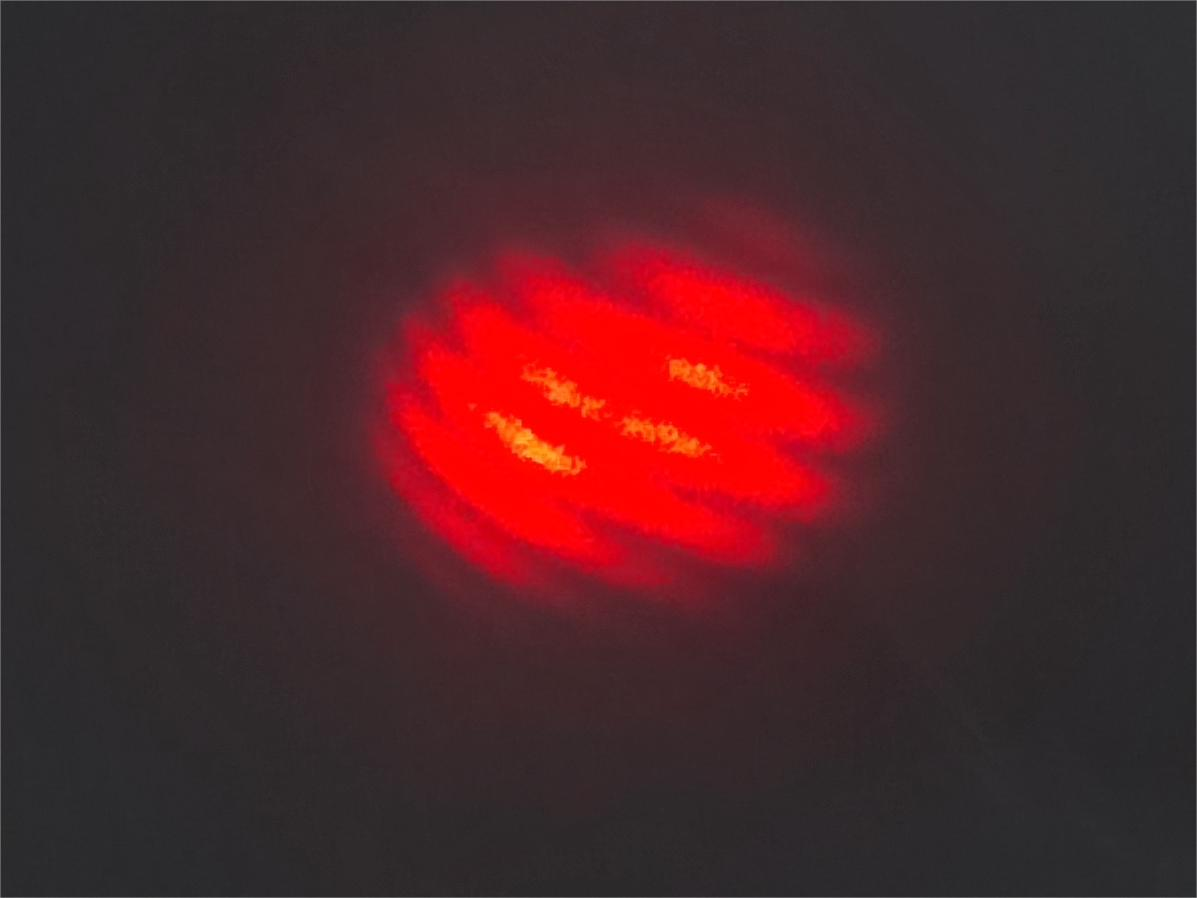
\includegraphics[width=5cm]{Fig/2.jpg}
        %        \caption{示波器显示-双波}
        %    \end{minipage}
        %    \begin{minipage}[t]{0.33\linewidth}
        %        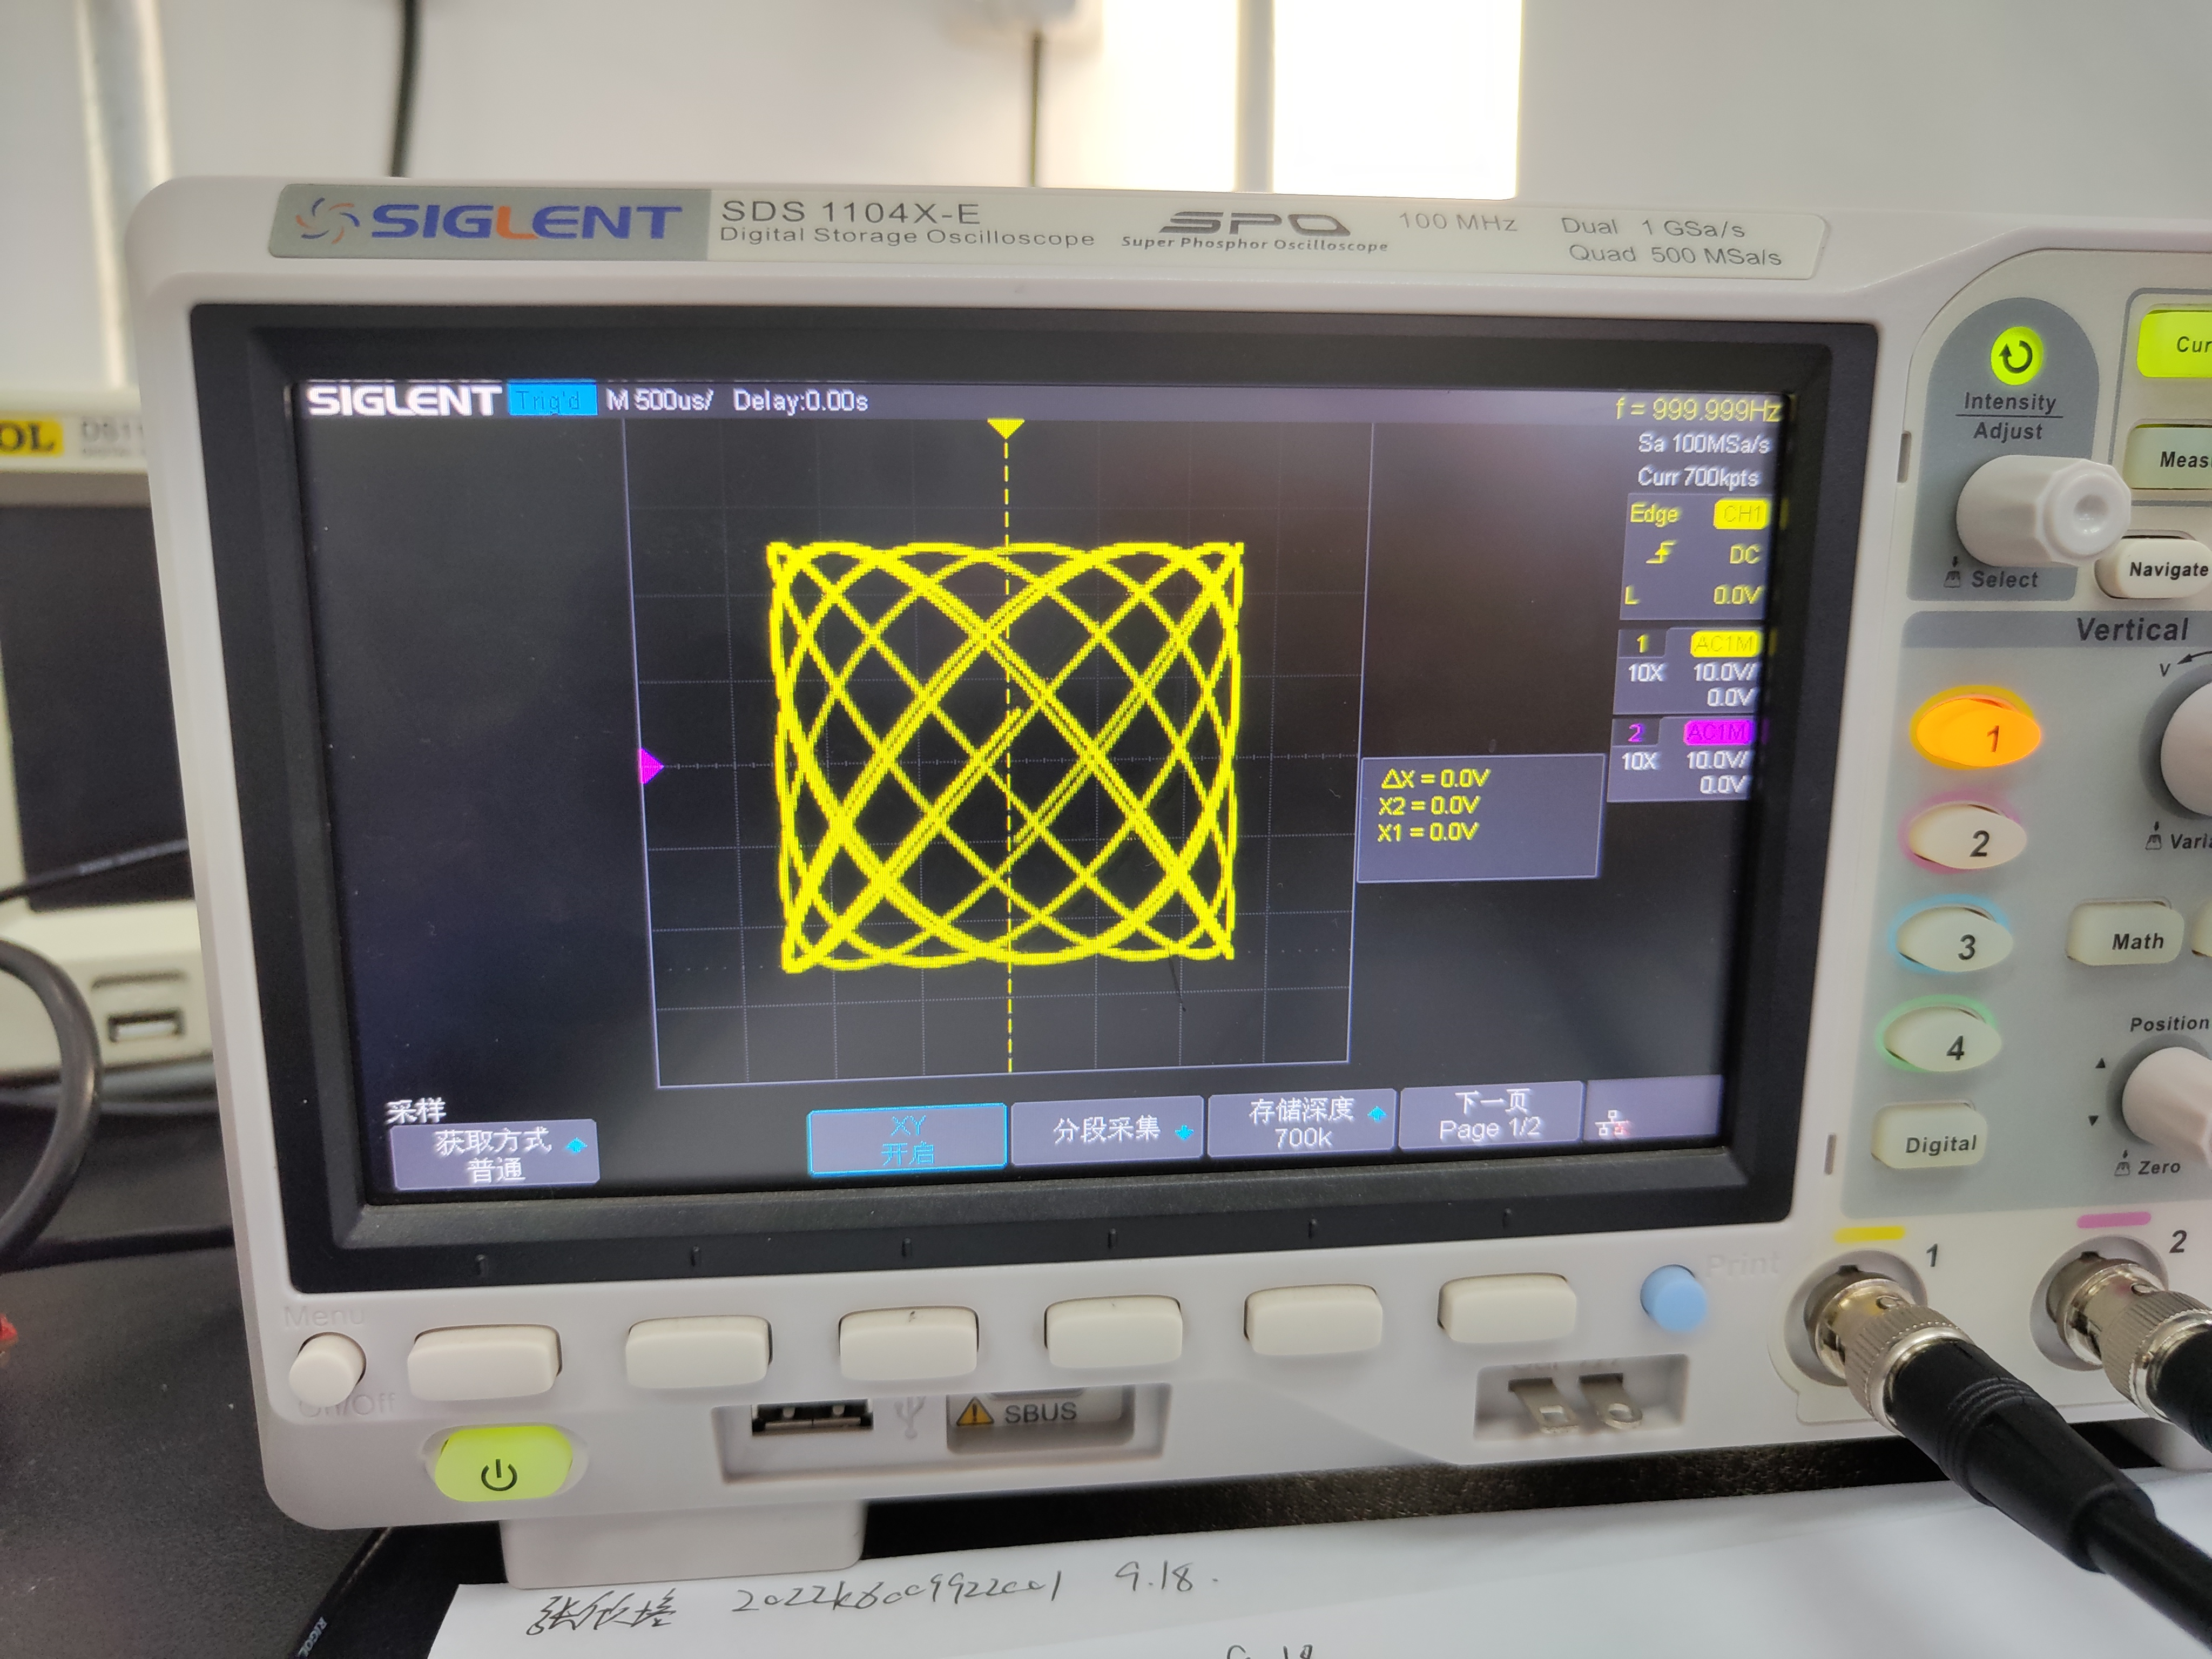
\includegraphics[width=5cm]{Fig/3.jpg}
        %        \caption{李萨如图像}
        %    \end{minipage}
        %    
        %\end{figure}

        \item 探头的使用,电容补偿,按规格调整衰减比。实际操作中,前人已完成调整,不太需要我去调整电容补偿,接入后图像较为平直。测量人体电压与波形,大致为正弦型波形,6V左右,50Hz。
        \item 使用电路板,观察一些电源输出的波形和其转换。
        \item 使用稳压电源点亮发光二极管,使用电表测量以计算阻值。1.7V左右亮,2.75V时0.10A,R=27.5Ω。
        \item 练习电表的使用,测量电阻阻值。
        
        %下面是图片
        %\begin{figure}[H]
        %    \centering
        %    \begin{minipage}[t]{0.33\linewidth}
        %        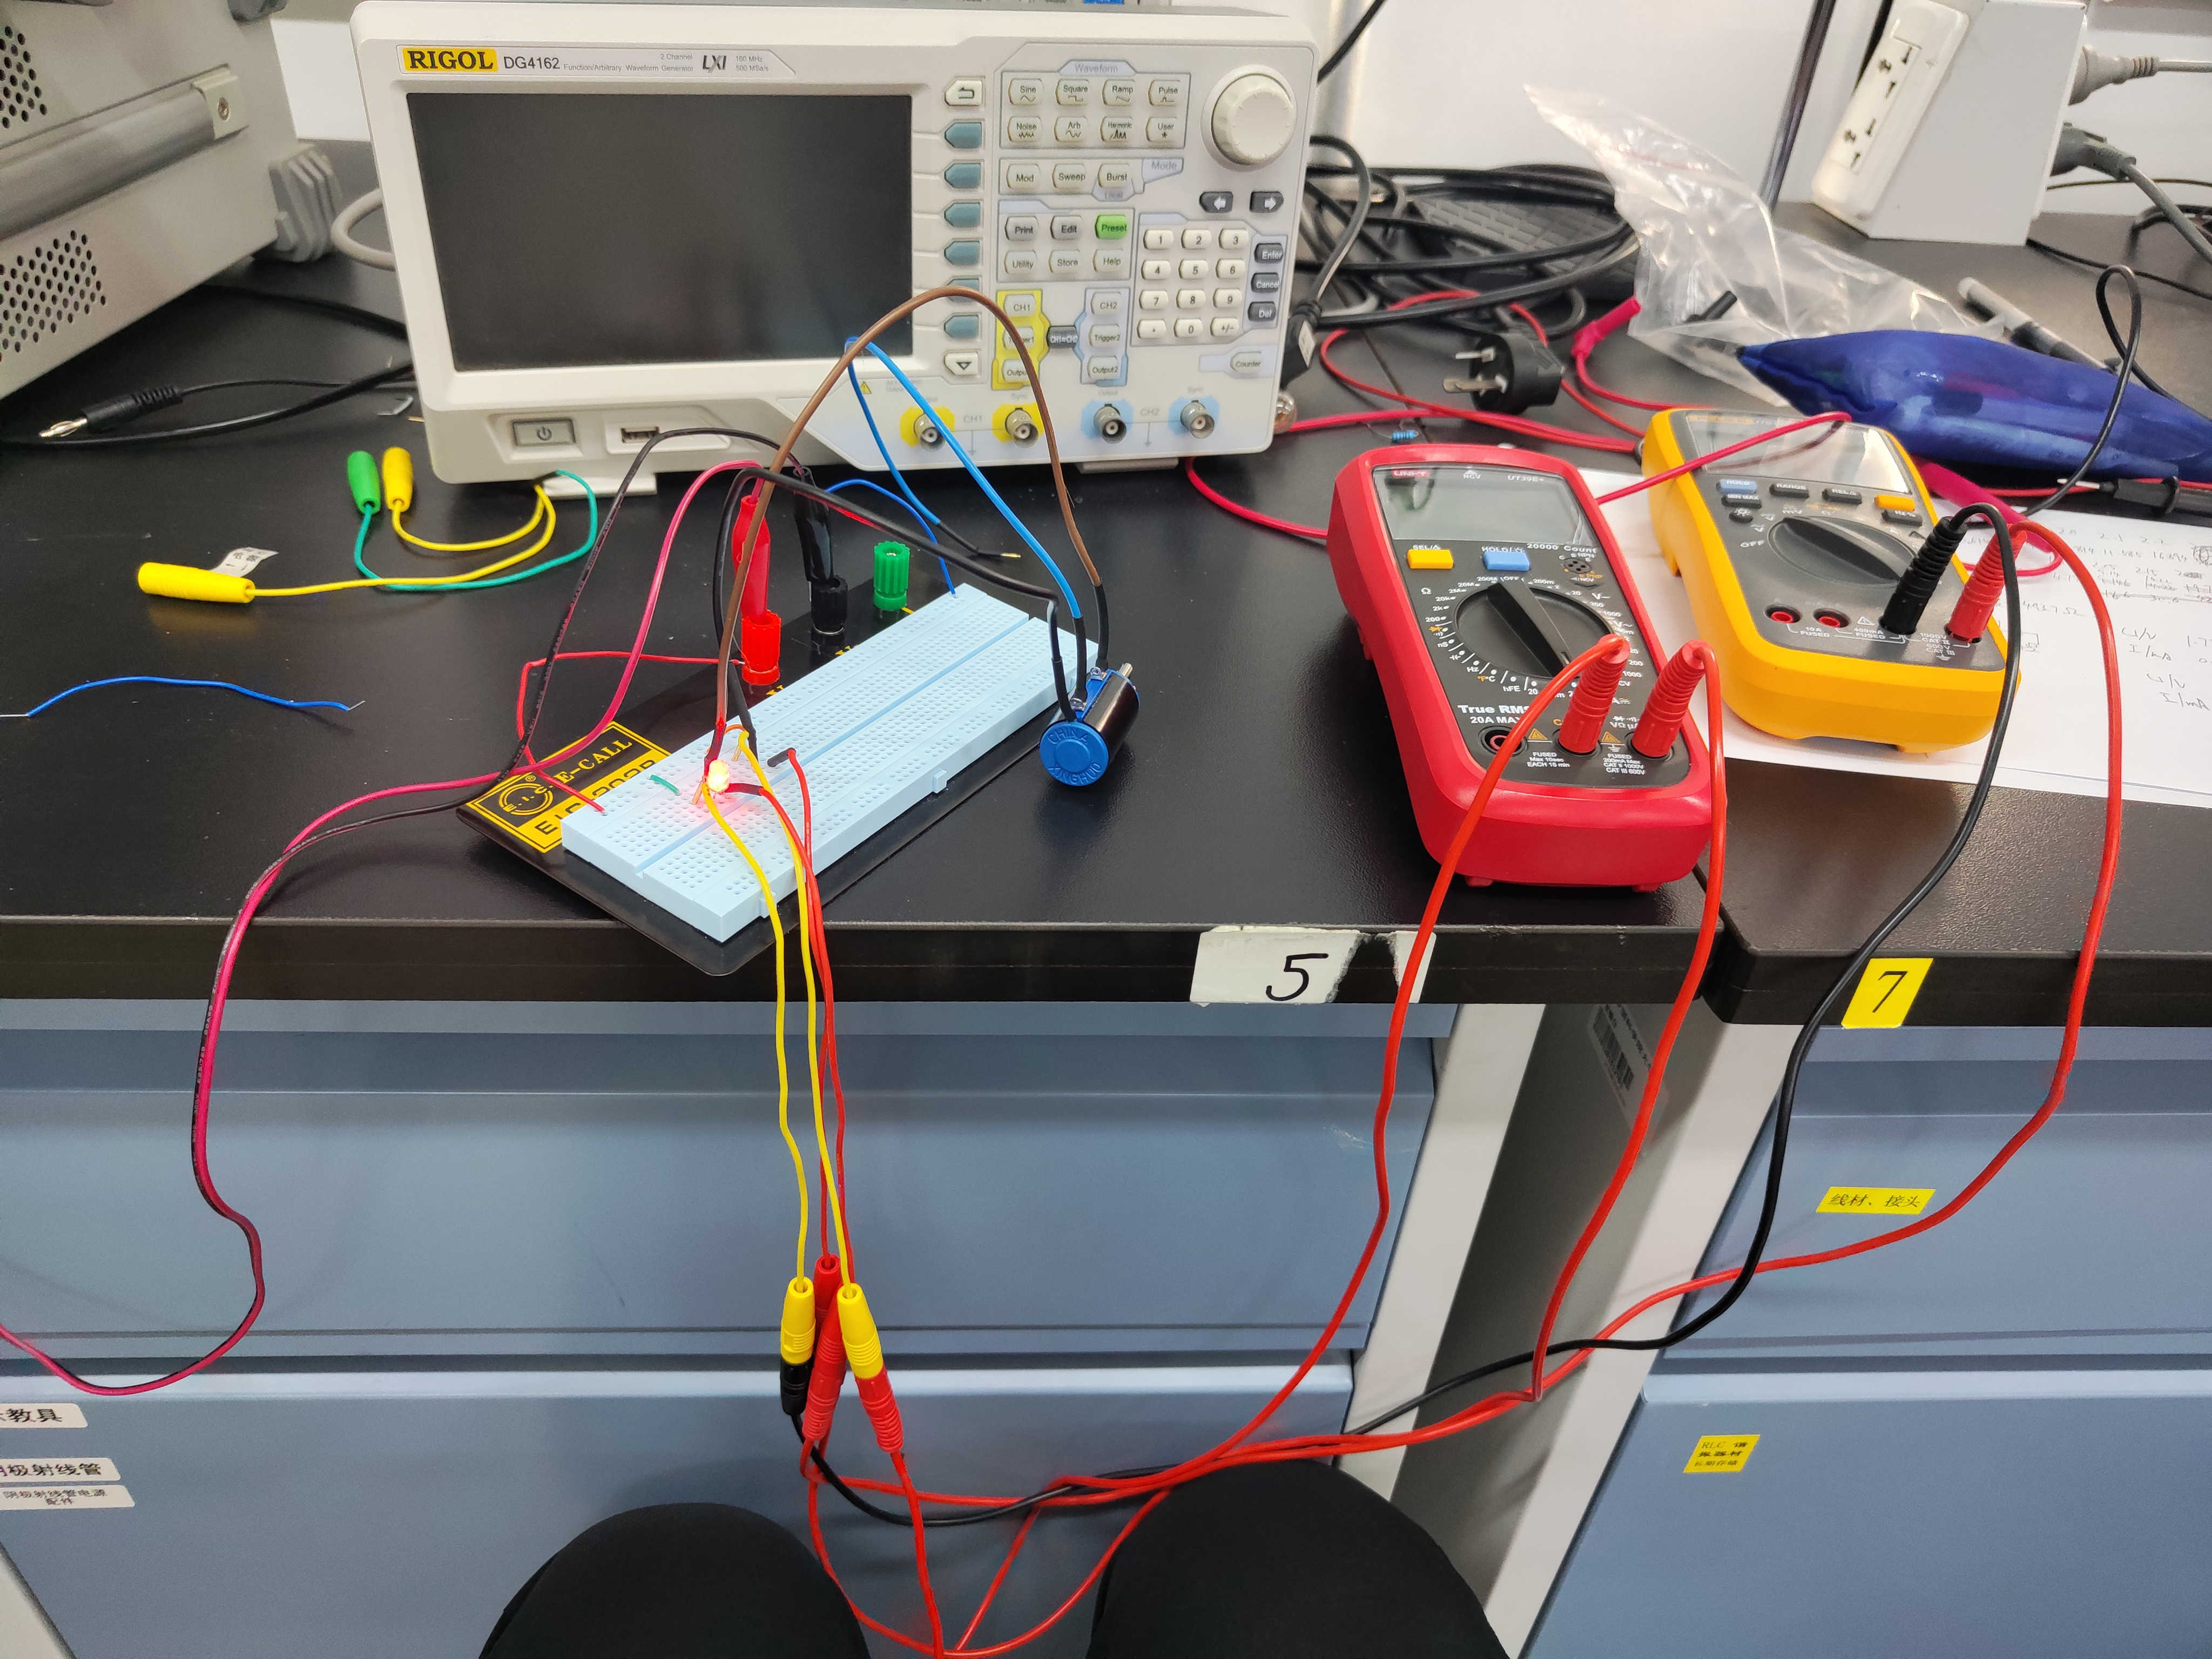
\includegraphics[width=5cm]{Fig/4.jpg}
        %        \caption{探头补偿}
        %    \end{minipage}
        %    \begin{minipage}[t]{0.33\linewidth}
        %        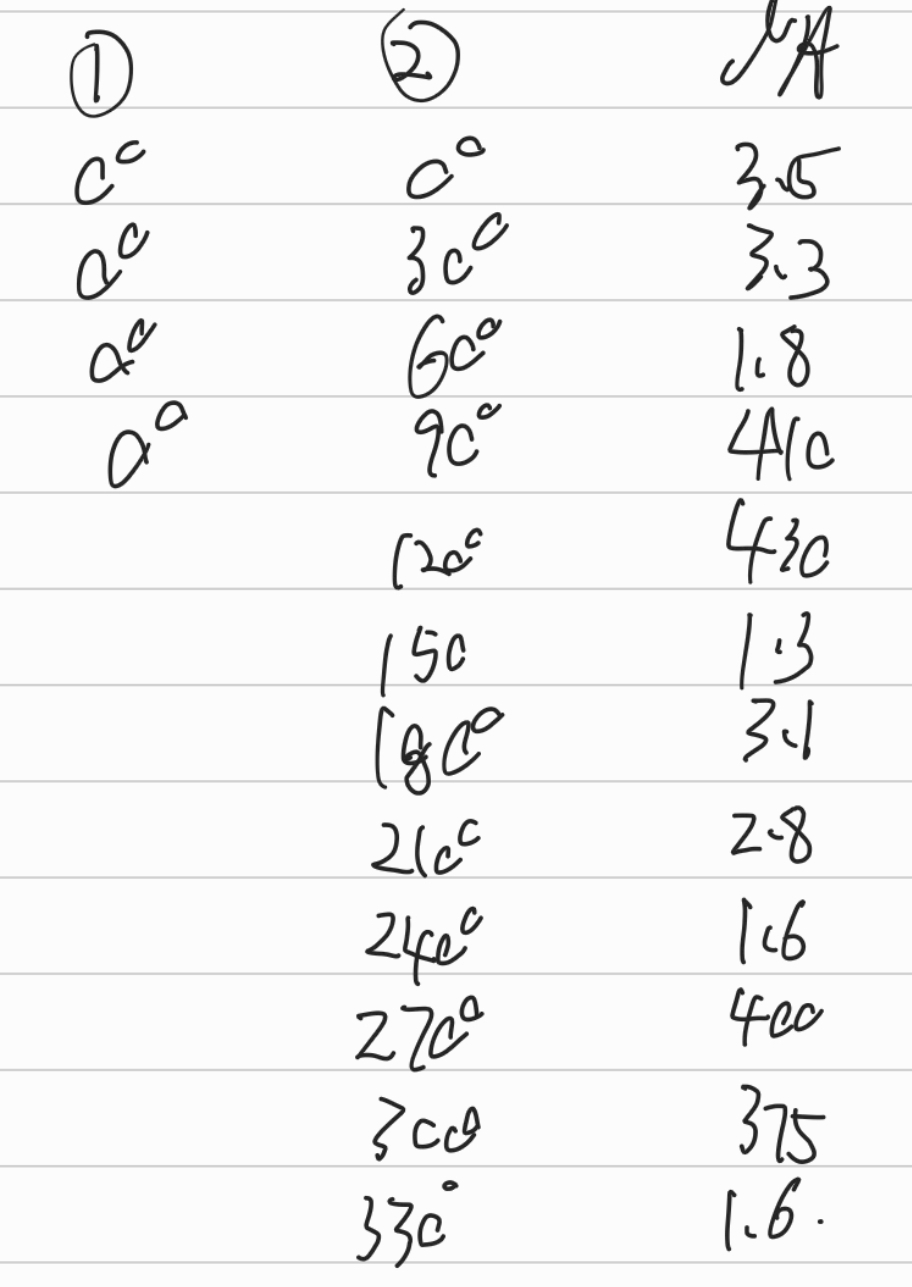
\includegraphics[width=5cm]{Fig/5.jpg}
        %        \caption{探头测量人体电压}
        %    \end{minipage}
        %    \begin{minipage}[t]{0.33\linewidth}
        %        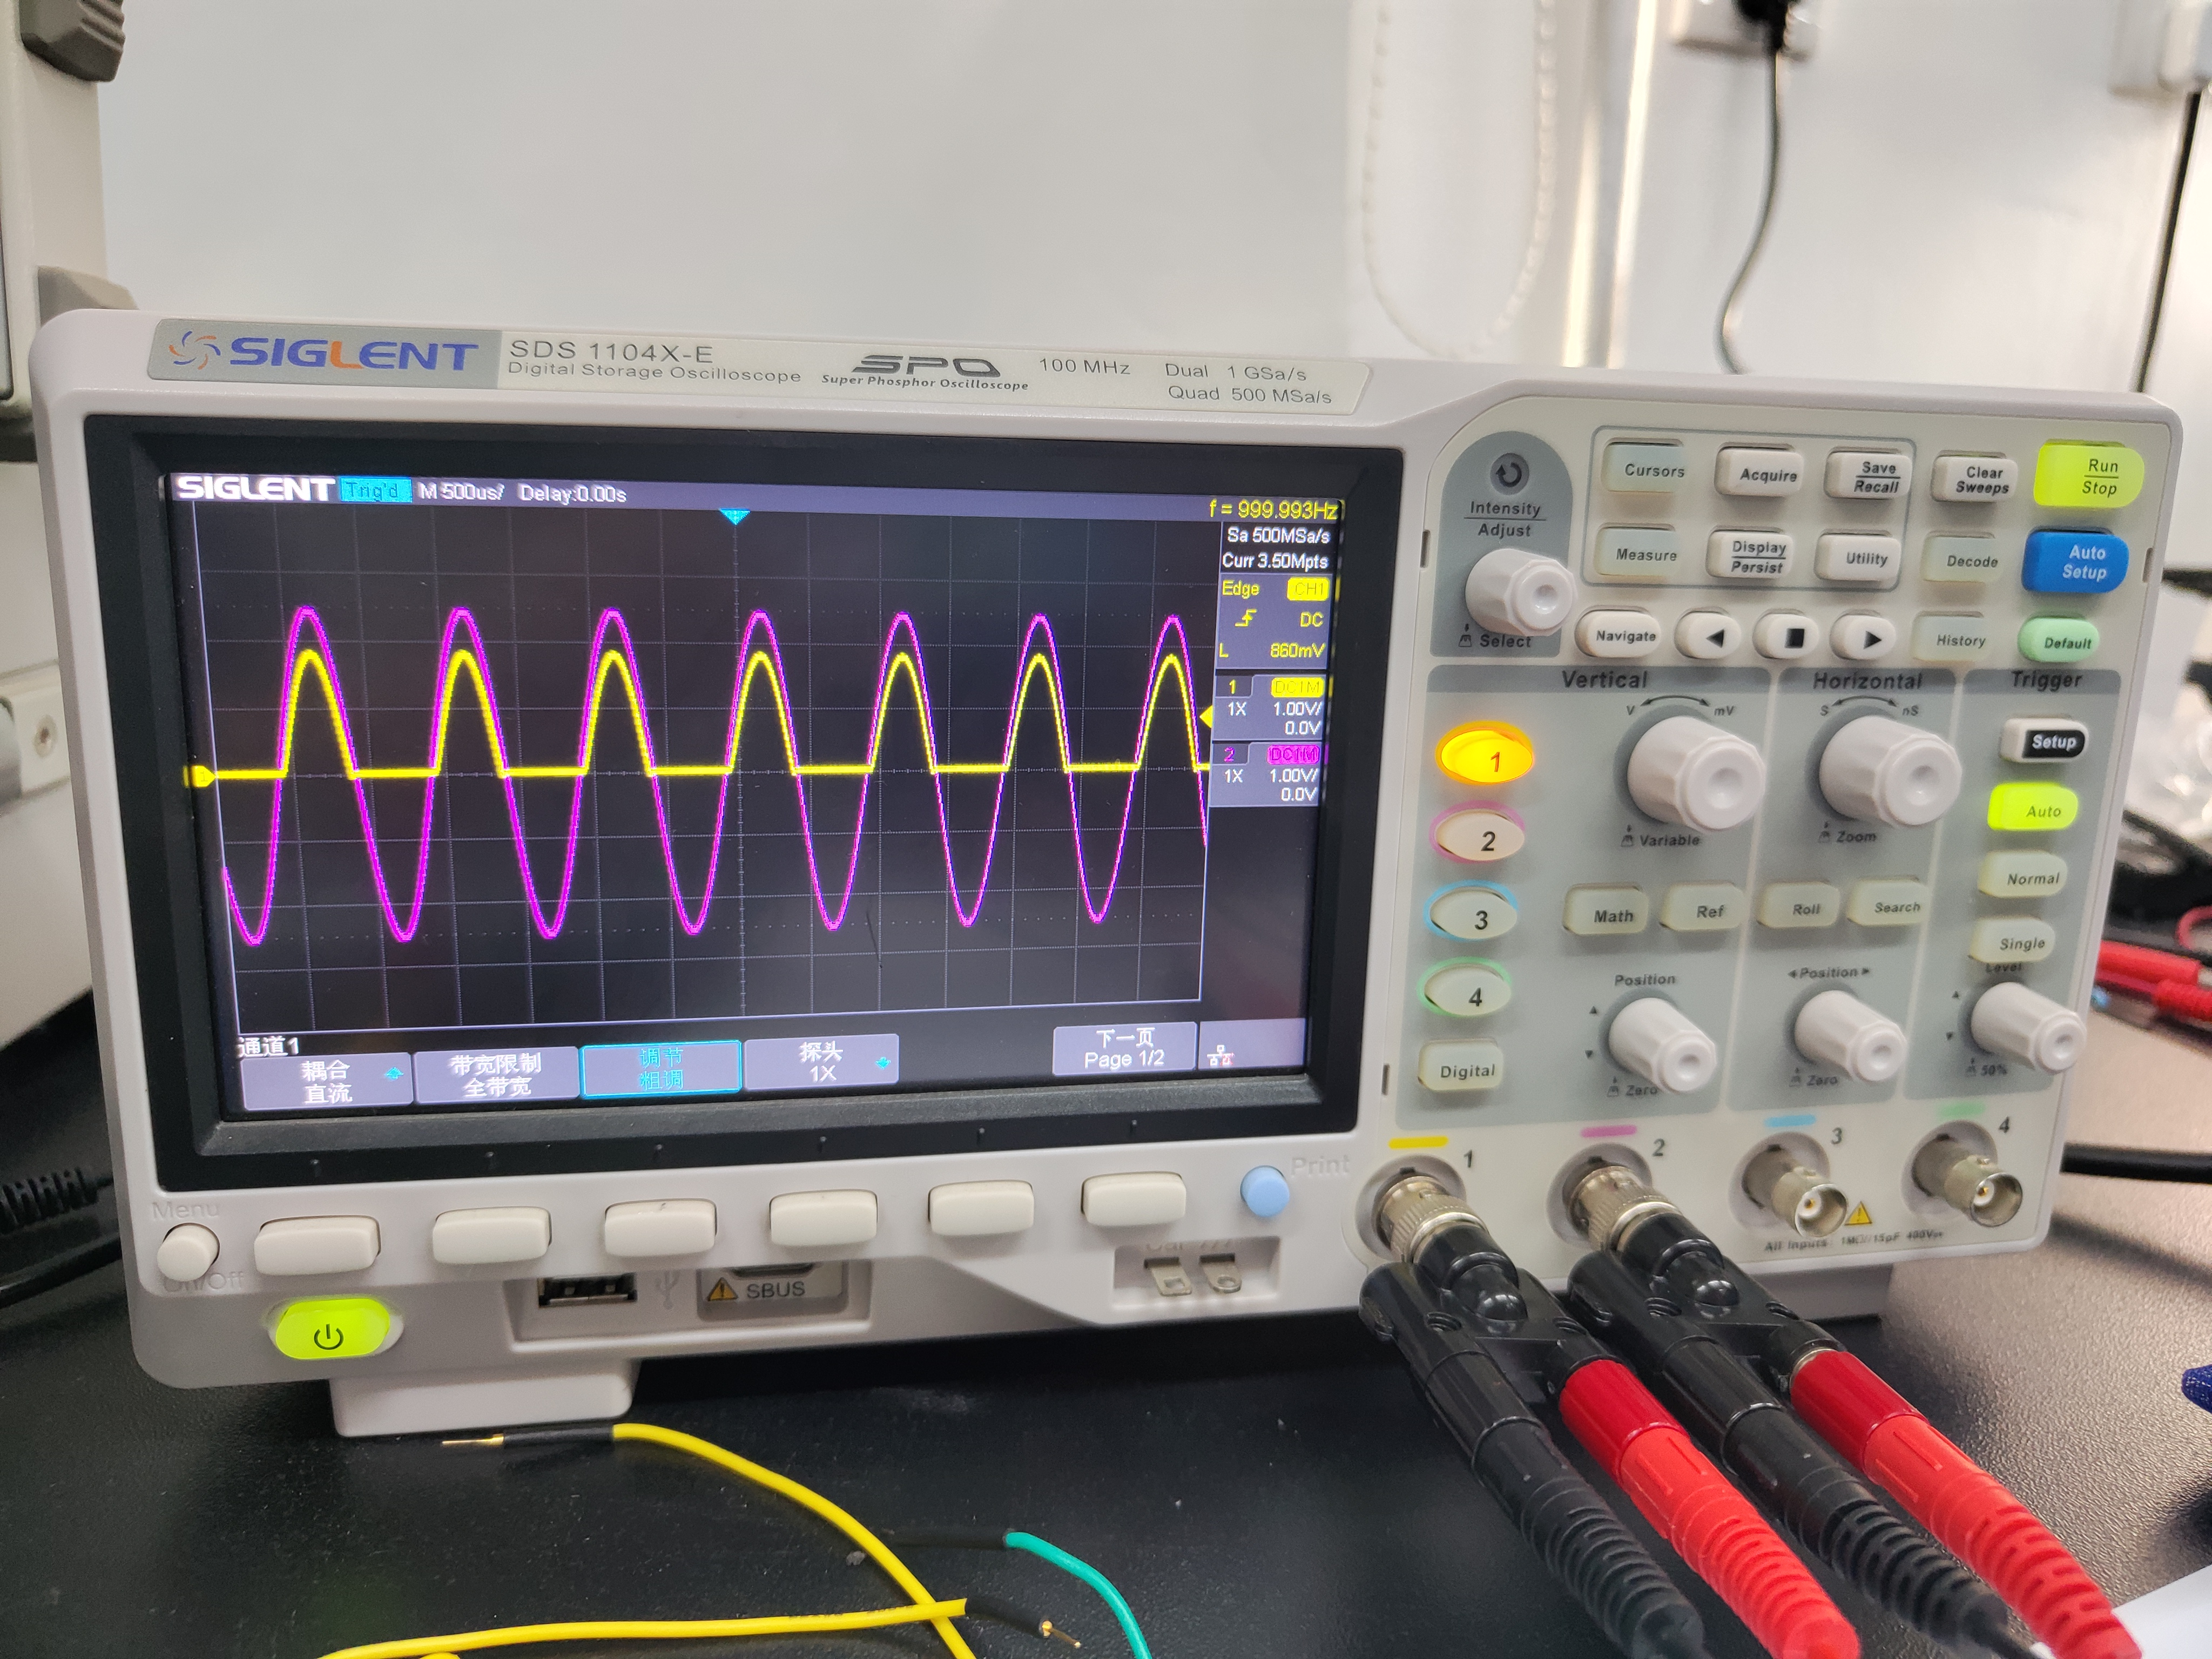
\includegraphics[width=5cm]{Fig/6.jpg}
        %        \caption{电源生成的脉冲波}
        %    \end{minipage}
        %    
        %\end{figure}

        %\begin{figure}[H]
        %    \centering
        %    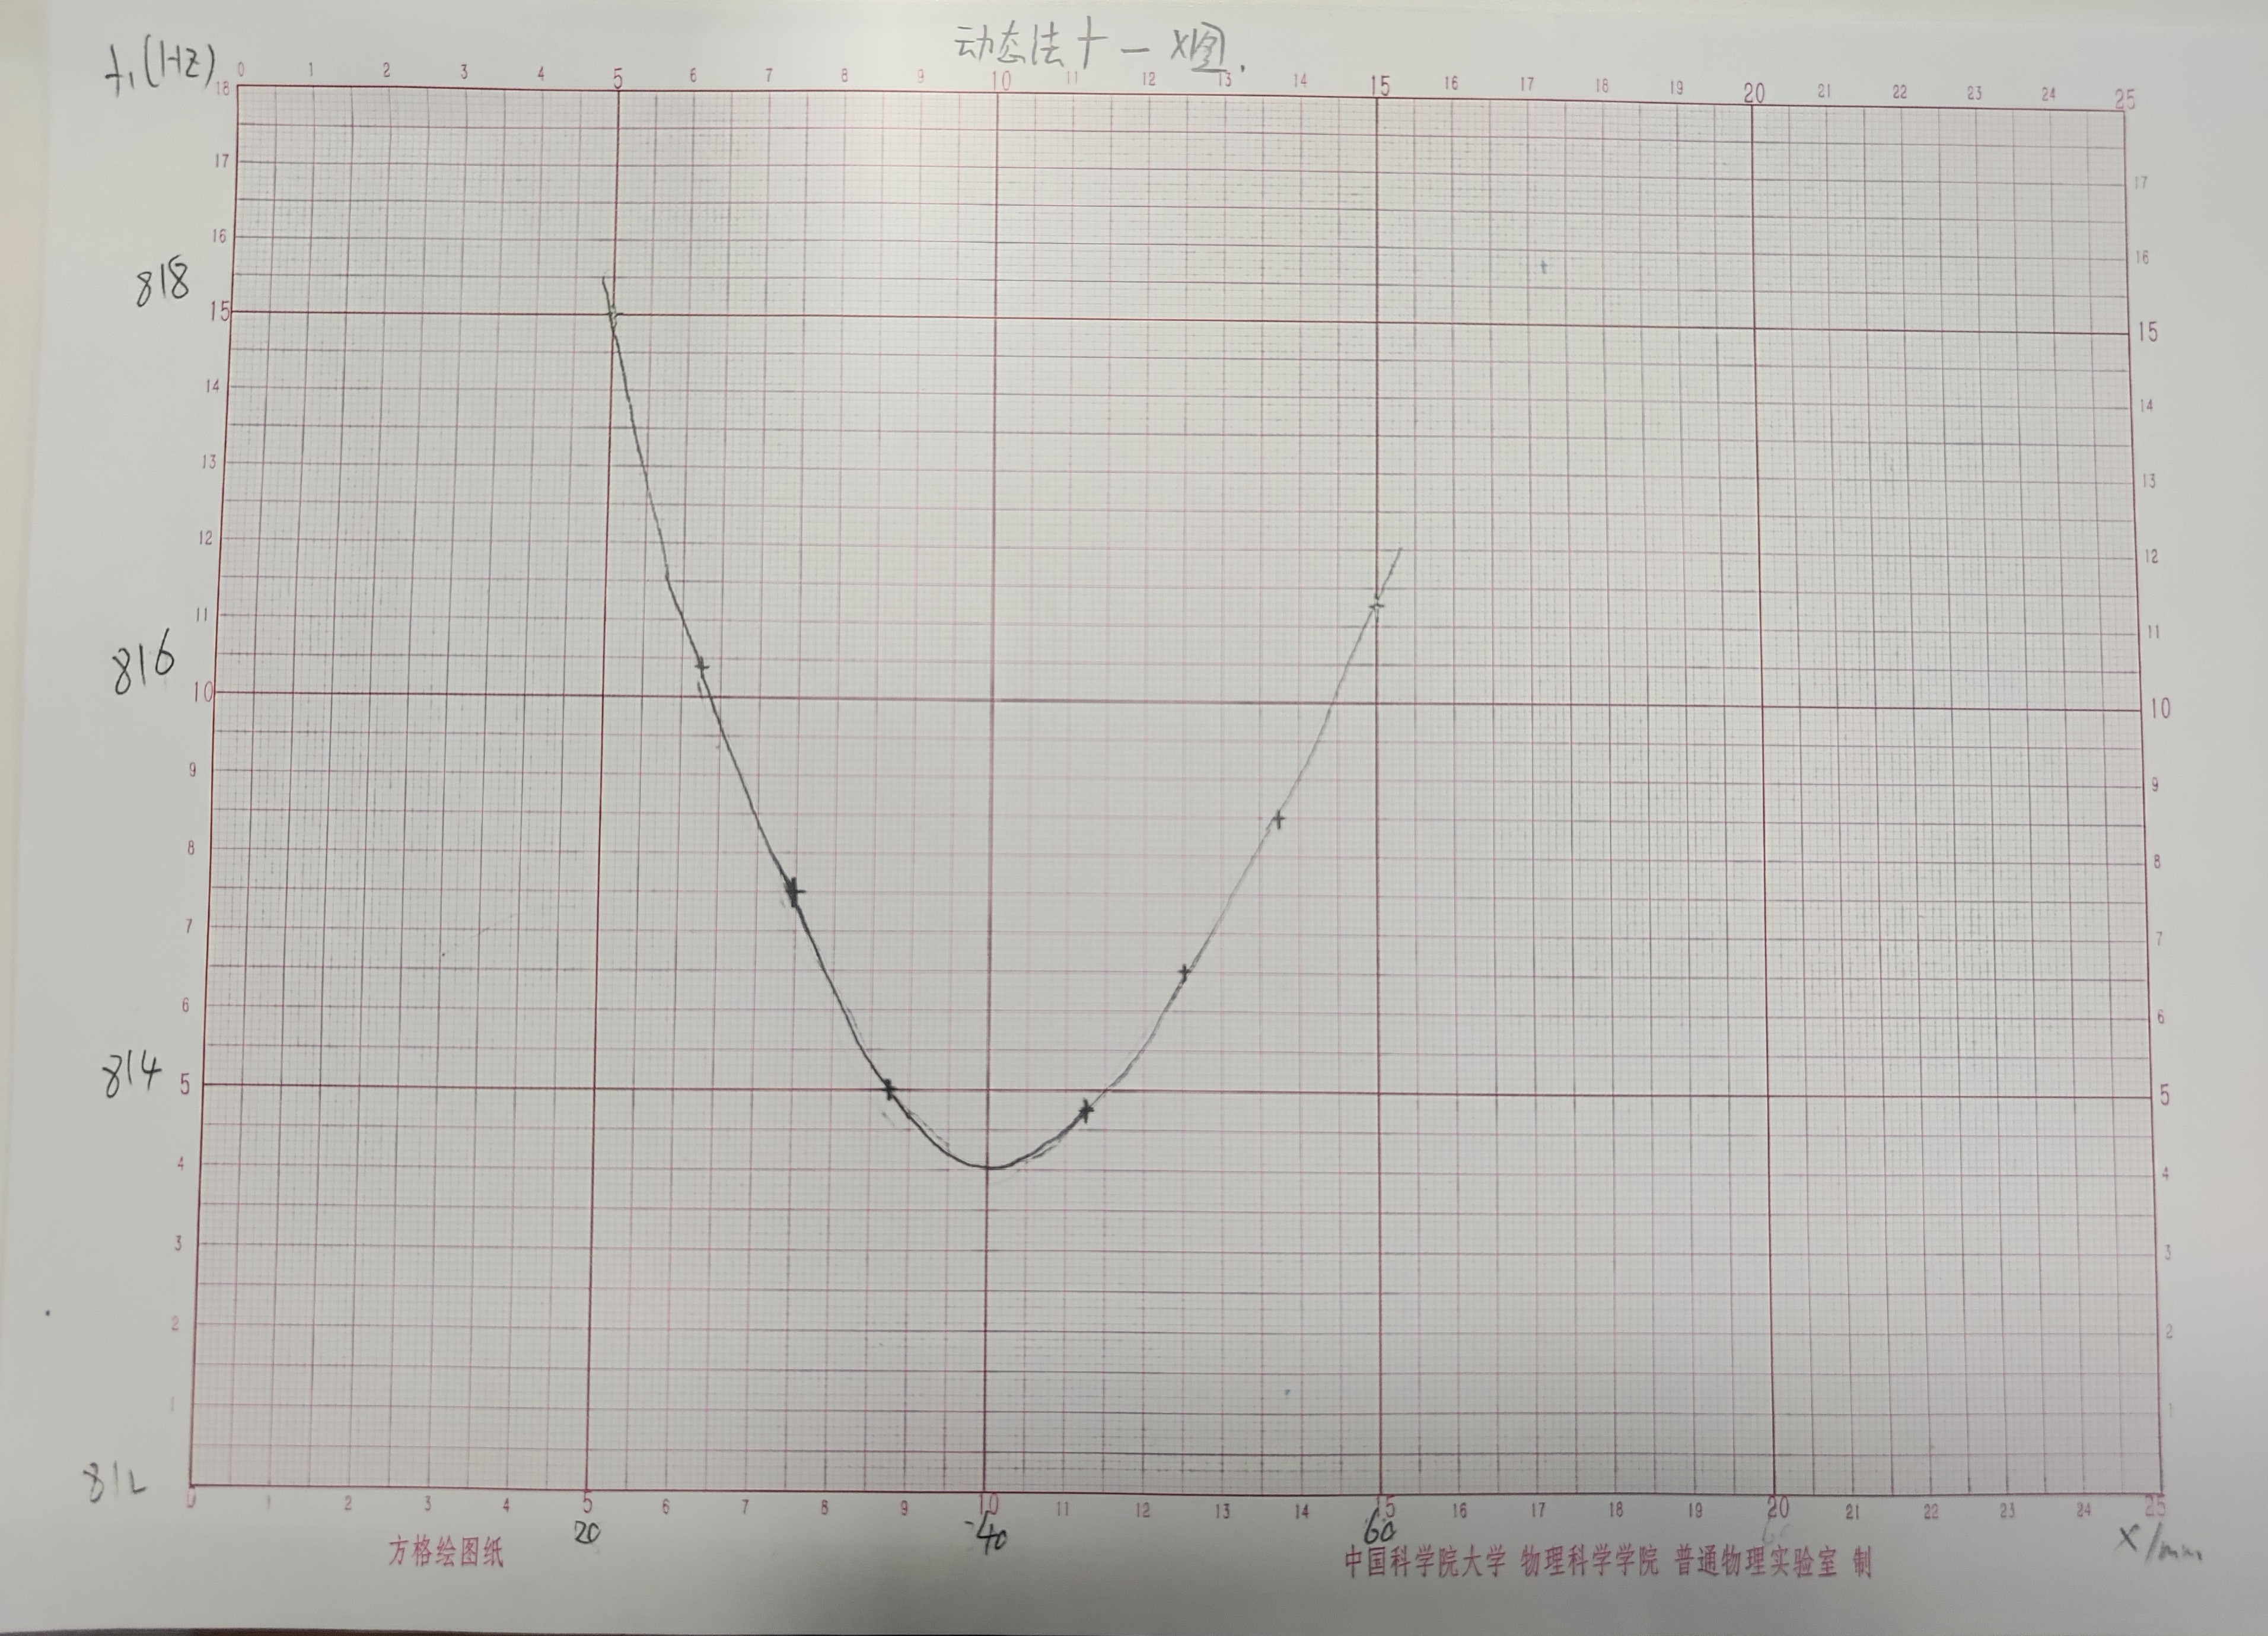
\includegraphics[width=6cm]{Fig/7.jpg}
        %    \caption{电表测电阻}
        %\end{figure}

    \end{enumerate}
\end{enumerate}

\section{实验反思、收获与总结}
\begin{enumerate}
    \item 示波器,信号发生器型号不同,操作不太一致,之后使用之前要先熟悉自己的设备。
    \item 示波器auto按键功能强大。
    \item 波的种类繁多,进行组合与变换以后更加多。
    \item 稳压电源输出电压基本恒定。
    \item 实验要及时记录和拍照。本次为我的第一次参与实验,最开始没有形成及时记录的习惯,只是在自己探索仪器使用方法,导致缺失了一些很漂亮的图像图片。未来不能再缺失图片。
\end{enumerate}


\begin{center}
    \vspace*{1em}
    \Large \bf 第二部分\qquad 实验原始记录
\end{center}

%\begin{figure}[H]
%    
%    \begin{minipage}[t]{1\linewidth}
%        \centering
%        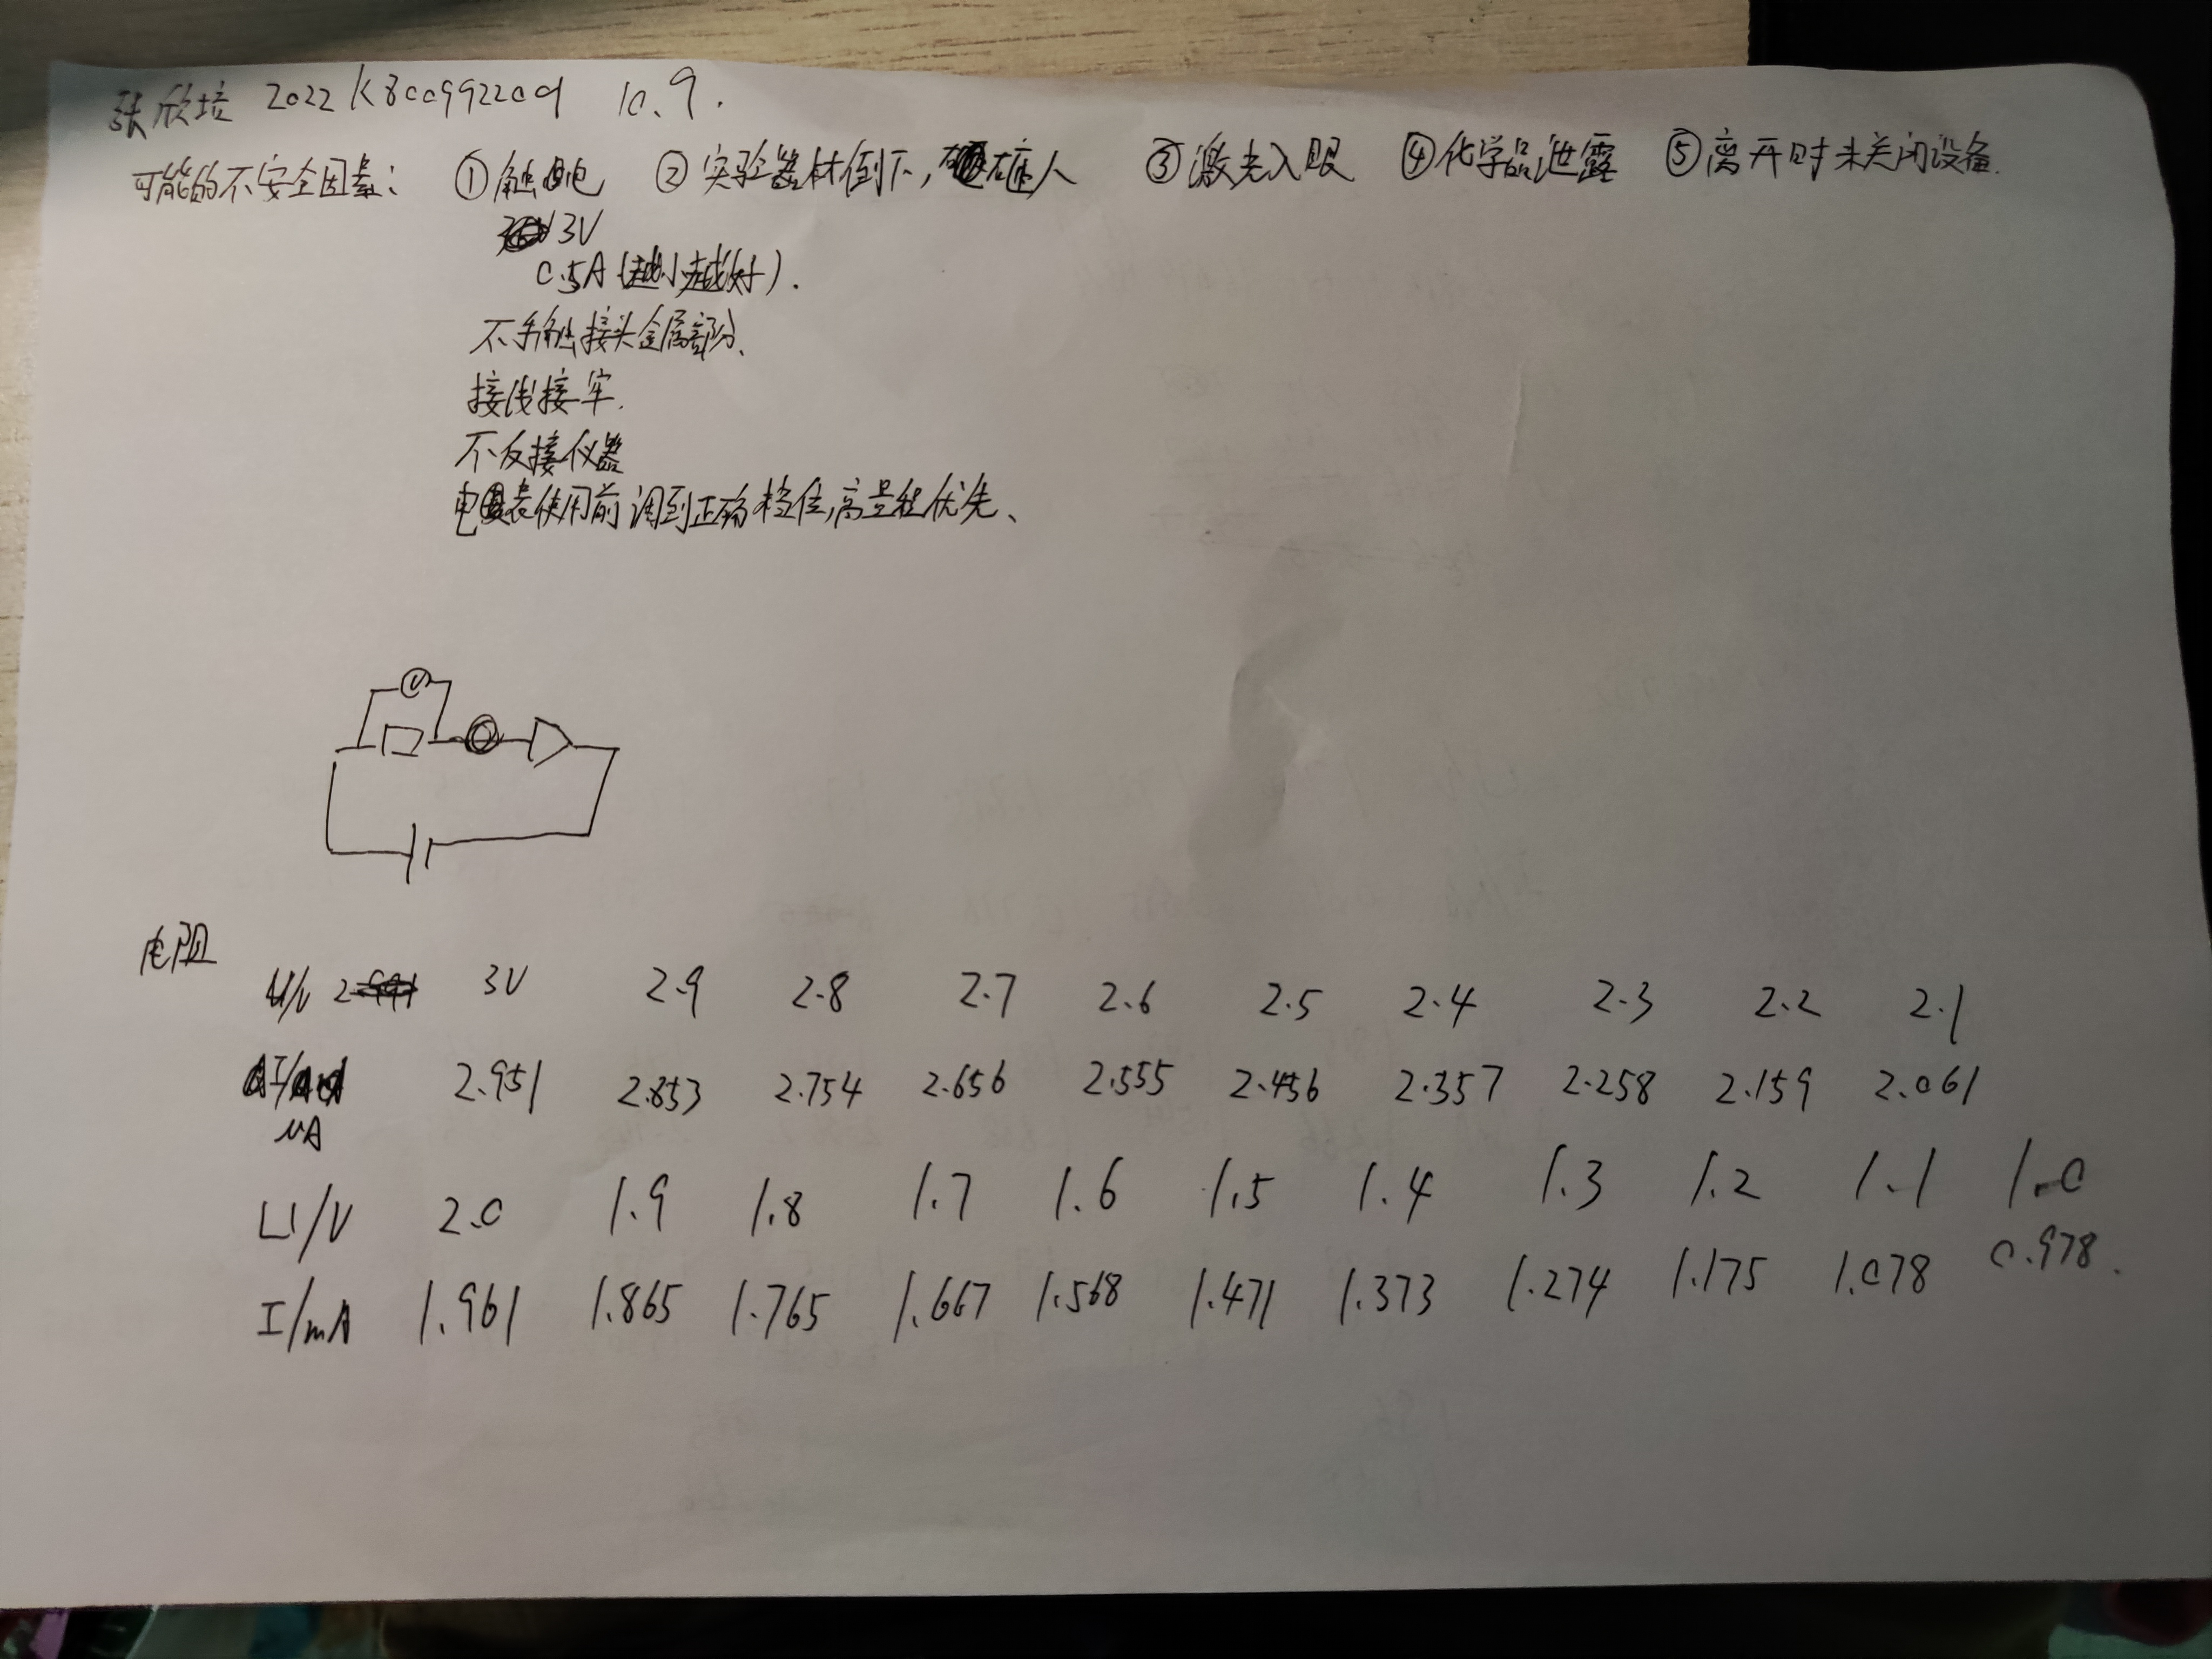
\includegraphics[width=15cm]{Fig/8.jpg}
%        \caption{实验原始记录1}
%        \vspace*{1em}
%    \end{minipage}
%    
%    \begin{minipage}[t]{1\linewidth}
%        \centering
%        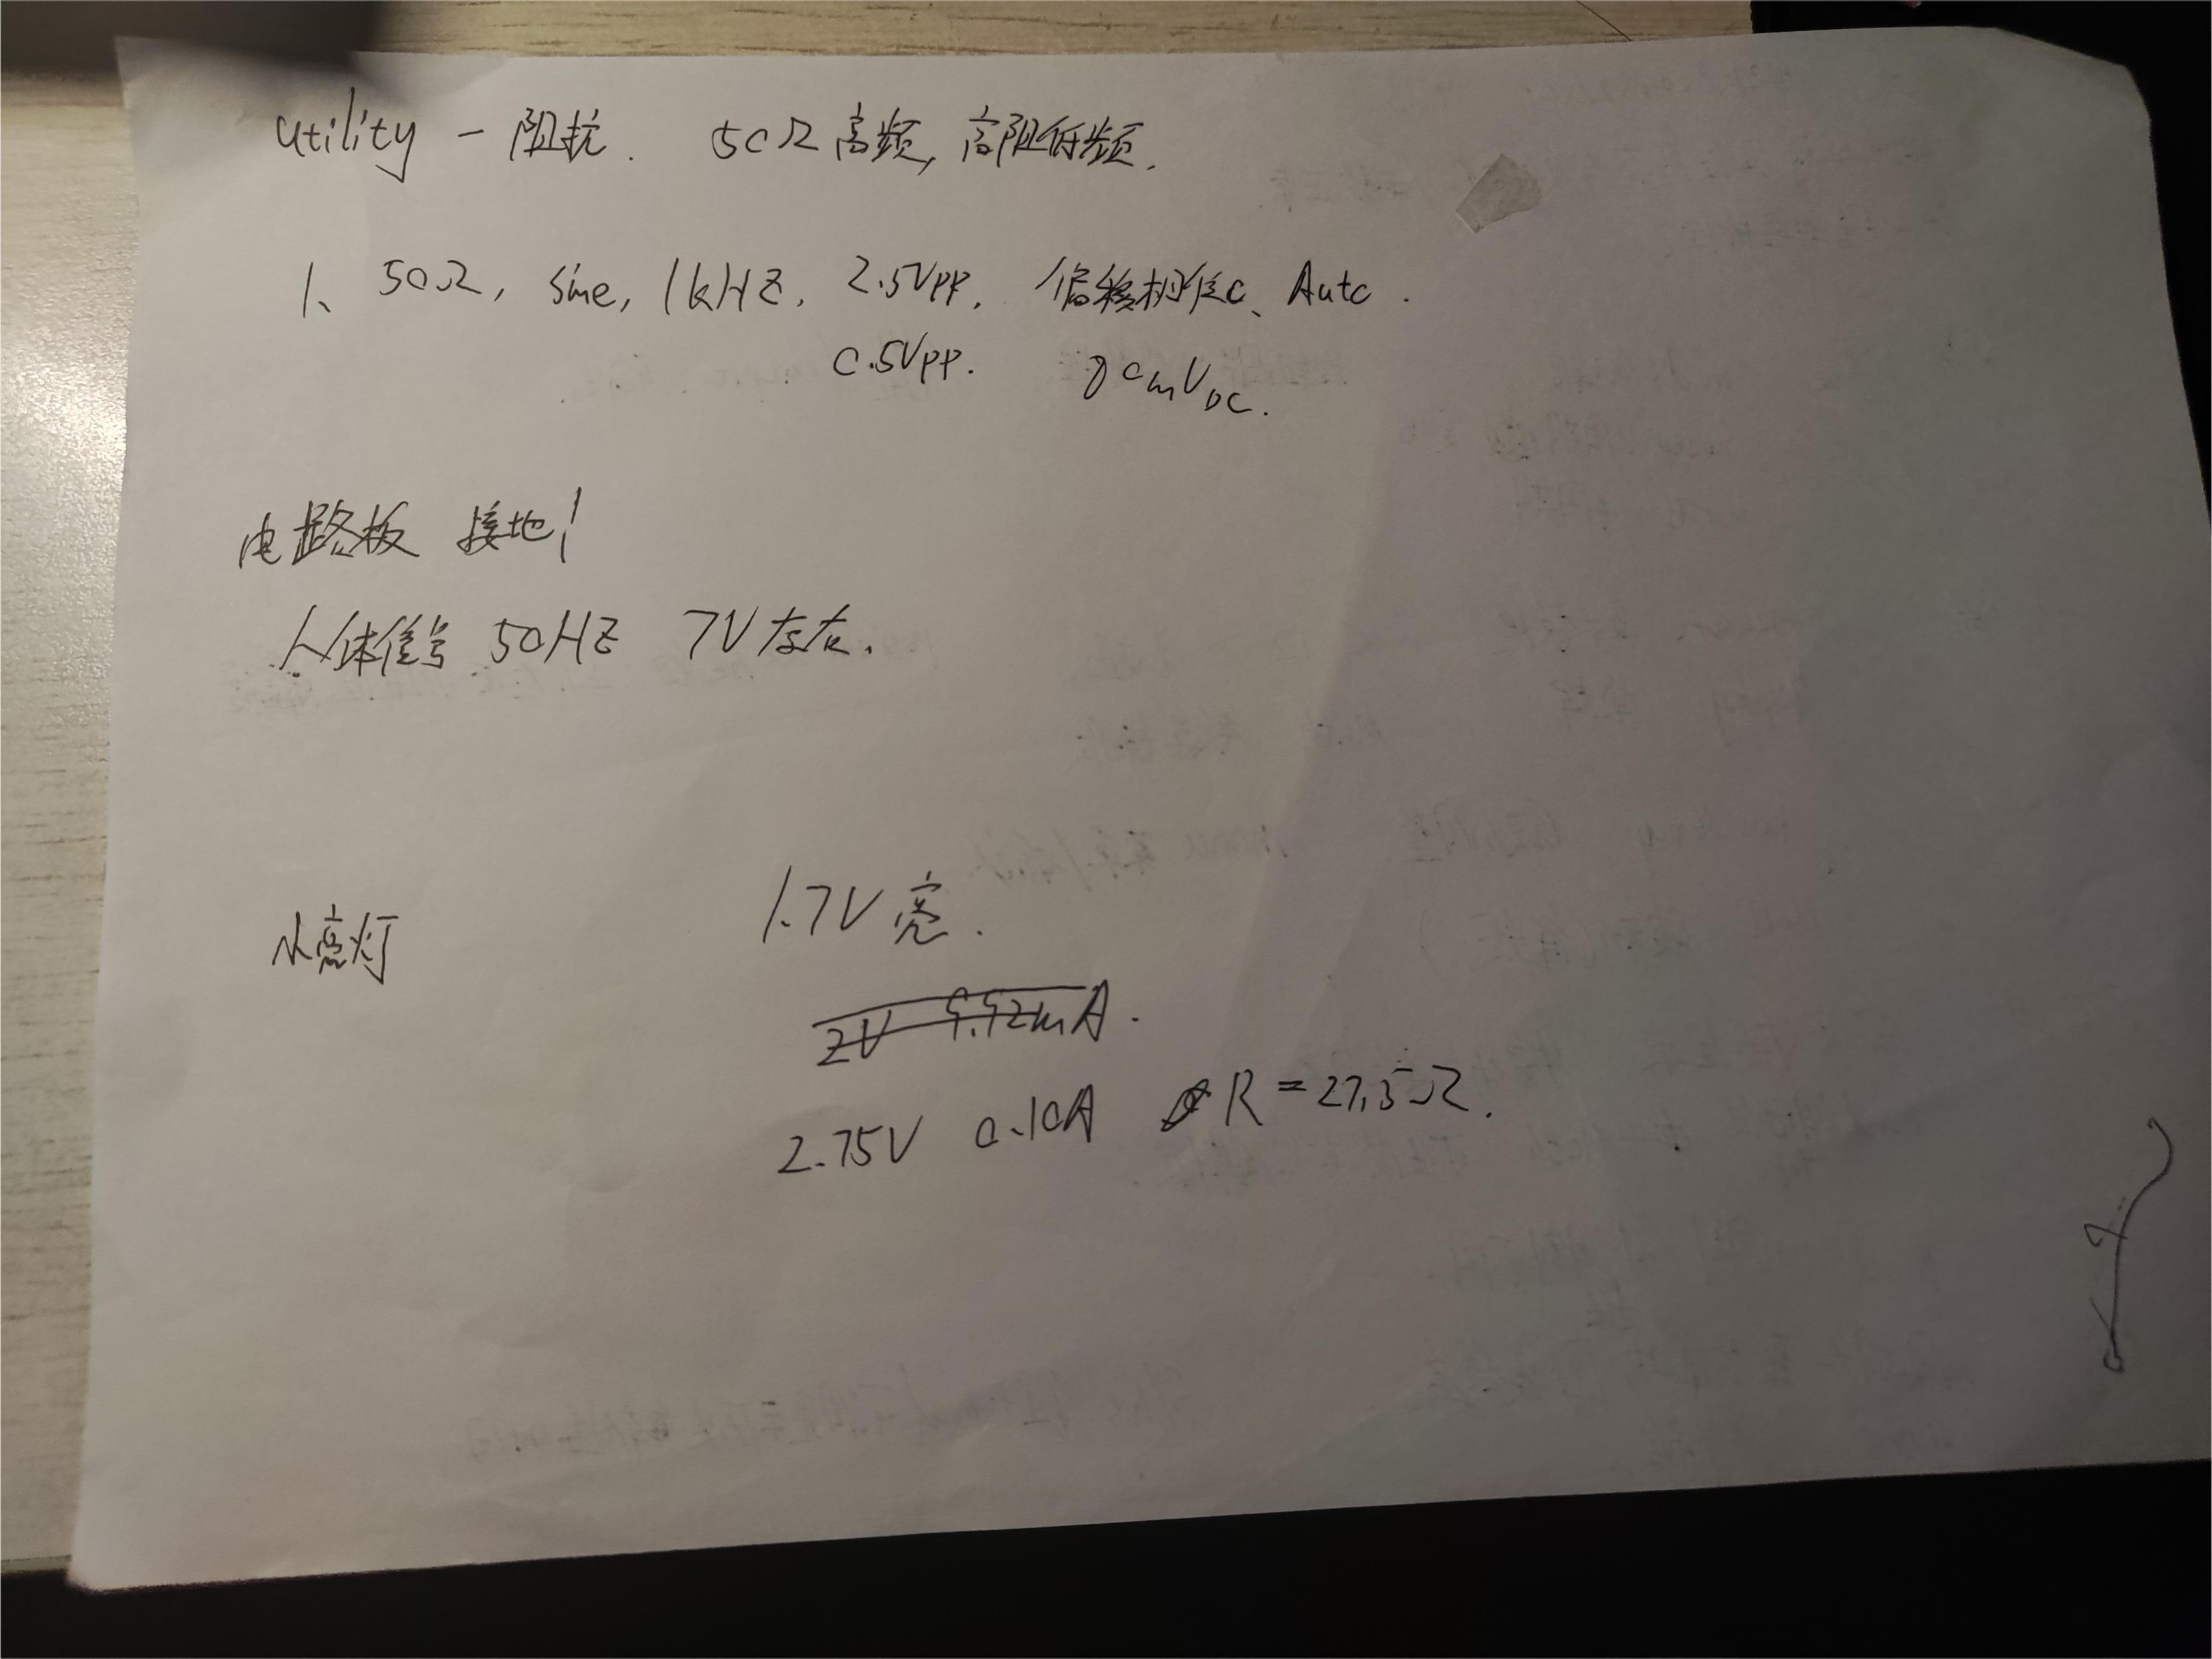
\includegraphics[width=15cm]{Fig/9.jpg}
%        \caption{实验原始记录2}
%        \vspace*{1em}
%    \end{minipage}
%\end{figure}

\end{document}